\section{Experiments}
\label{sec:experiments}

\subsection{Experiment Setup}

We conduct all the experiments based on the customized MuJoCo Walker2D environment \cite{todorov2012mujoco}. The walker is a two-dimensional two-legged figure that consist of seven main body parts: a single torso at the top, two thighs in the middle below the torso, two legs in the bottom below the thighs, and two feet attached to the legs on which the entire body rests. The goal is to walk or run in the in the forward direction by applying torques on the six hinges connecting the seven body parts. The state space and the action space contain $24$ and $6$ dimensions respectively. The two tasks have exactly the same state space, action space and transition probability. The only difference is the reward function.

The dataset consists of offline samples from two tasks (i.e. \texttt{walk} and \texttt{run}), each including two data quality levels (i.e. \texttt{medium} and \texttt{medium-replay}). They are collected from the replay buffer when training an online TD3 agent. In this project, the agent can only learn from the offline dataset when training while the evaluation is conducted online \cite{fu2020d4rl}. We expect the multi-task agent to learn from all the samples in the dataset and achieve satisfactory performance in both tasks.

According to Section \ref{sec:method}, we implement three algorithms step by step: conservative soft actor-critic (CSAC), multi-task conservative soft actor-critic (MTCSAC), and heuristic conservative soft actor-critic (HCSAC). CSAC is the classic conservative Q-learning (CQL) algorithm based on the soft actor-critic (SAC) framework. MTCSAC adds the task embedding based on CSAC, which can realize multi-task learning. HCSAC further introduces the heuristic relabeling method to extend the offline dataset, which may further improve the performance of MTCSAC. All the critic and actor networks are implemented as multi-layer perceptrons (MLPs) \cite{rumelhart1986learning} with $3$ hidden layers and $1024$ hidden units. The output action is mapped to the range $(-1, 1)$ by a $\tanh$ function.

The experiments are divided into two groups (i.e. \texttt{medium} and \texttt{medium-replay}) according to the dataset used for training. In each group, CSAC is trained on the two tasks (i.e. \texttt{walk} and \texttt{run}) separately, while MTCSAC and HCSAC are trained on the union of the datasets for the two tasks. All the agents are trained for $1000$ epochs with a batch size of $1024$. Online evaluation is conducted every $10$ epochs. Heuristic relabeling is conducted every $100$ epochs for HCSAC. We use the Adam algorithm \cite{kingma2014adam} to optimize the neural networks, where the learning rate is set to $3\times 10^{-4}$ for the critic and $1\times 10^{-4}$ fot the actor. The soft update rate is set to $0.01$ to update the target networks. The discount factor is set to $0.99$. The weight of the CQL loss term is set to $10.0$. We sample $10$ actions each from the uniform distribution and the policy distribution to estimate the log-sum-exp term in the CQL loss. The quantile is set to $5\%$ in the heuristic relabeling algorithm for HCSAC.

\subsection{Performance Evaluation}

\begin{figure}[ht]
    \centering
    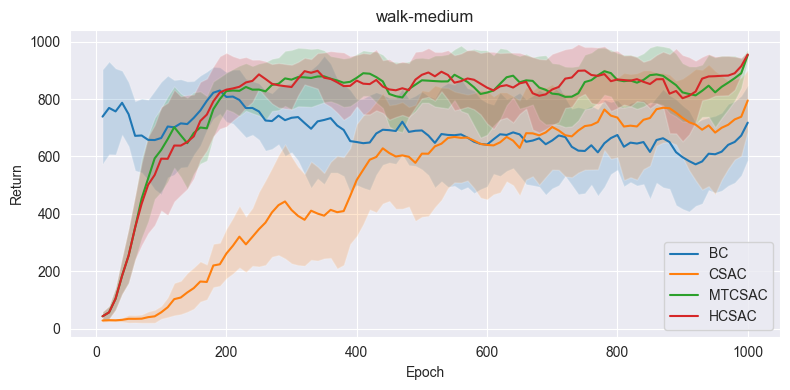
\includegraphics[width=0.45\textwidth]{figure/walk_medium.png}
    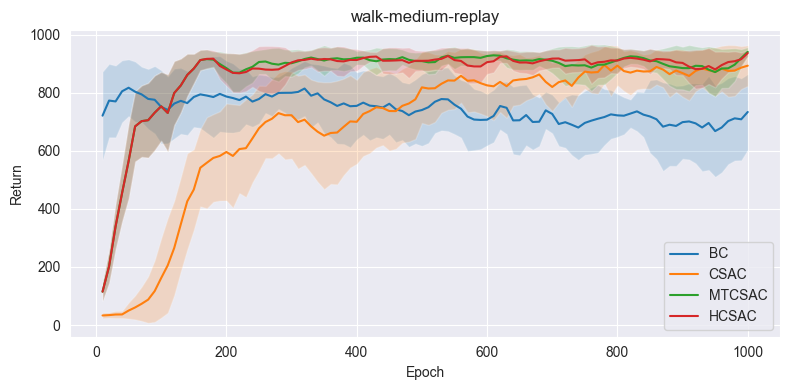
\includegraphics[width=0.45\textwidth]{figure/walk_medium_replay.png}
    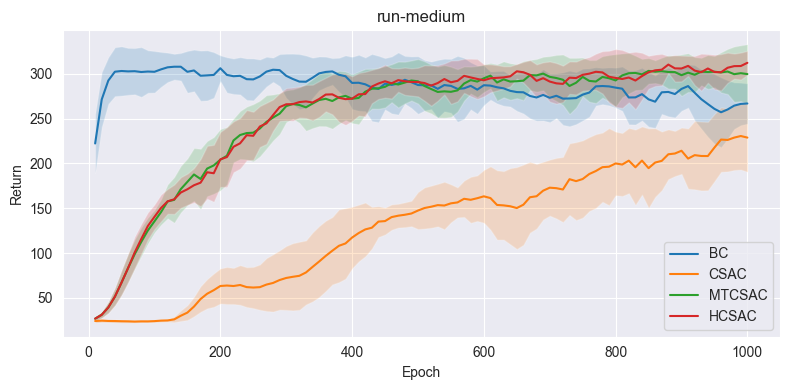
\includegraphics[width=0.45\textwidth]{figure/run_medium.png}
    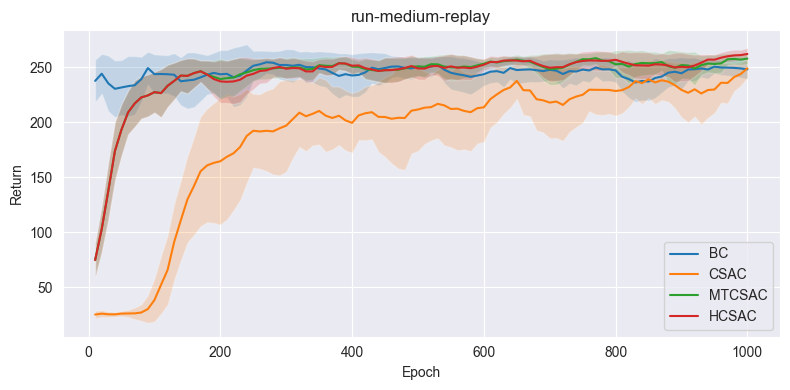
\includegraphics[width=0.45\textwidth]{figure/run_medium_replay.png}
    \caption{Training curves of the agents on the Walker2D environment. The top row shows the results of the \texttt{walk} task and the bottom row shows the results of the \texttt{run} task. The left column shows the results of the \texttt{medium} dataset and the right column shows the results of the \texttt{medium-replay} dataset.}
    \label{fig:experiment_result}
\end{figure}

Figure \ref{fig:experiment_result} shows the training curves of the agents on the Walker2D environment. We can see that MTCSAC (green curve) and HCSAC (red curve) significantly outperform CSAC (orange curve) in all the tasks, which demonstrates that the multi-task setting benefits the training process so that the agent can learn useful shared representations from different tasks. HCSAC performs slightly better than MTCSAC in majority of the training process, especially for the \texttt{medium} quality dataset, which indicates that the heuristic relabeling method can effectively augment the offline dataset so that the agent can learn from more valuable transitions. We can expect that HCSAC will achieve even better performance on the dataset with higher quality. The averages return in the \texttt{run} task are much lower than those in the \texttt{walk} task because the former is more challenging and requires precise control, which is consistent with the sampled trajectories in the offline dataset.

\begin{table}[ht]
    \caption{Performance evaluation of the agents on the Walker2D environment. The experiments are divided into two groups according to the dataset used for training, each containing two tasks. Every single experiment is conducted with $5$ different random seeds and the returns are reported in the form of mean and standard deviation. The best results are highlighted in bold.}
    \label{tab:performance_evaluation}
    \centering
    {\small \begin{tabular}{cccccc}
        \toprule
        \textbf{Dataset} & \textbf{Task} & \textbf{BC} & \textbf{CSAC} & \textbf{MTCSAC} & \textbf{HCSAC} \\
        \midrule
        \multirow{3}{*}{\texttt{medium}} & \texttt{walk} & $551.52 \pm 125.24$ & $653.57 \pm 233.83$ & $870.06 \pm 92.99$ & $\bm{907.38 \pm 67.39}$ \\
        & \texttt{run} & $\bm{317.26 \pm 9.46}$ & $213.67 \pm 49.56$ & $306.16 \pm 20.43$ & $308.38 \pm 7.64$ \\
        & \texttt{average} & $434.39 \pm 67.35$ & $433.62 \pm 141.70$ & $588.11 \pm 56.71$ & $\bm{607.88 \pm 37.52}$ \\
        \midrule
        \multirow{3}{*}{\texttt{replay}} & \texttt{walk} & $829.63 \pm 74.64$ & $812.80 \pm 146.82$ & $\bm{931.37 \pm 9.21}$ & $927.43 \pm 14.76$ \\
        & \texttt{run} & $244.80 \pm 33.35$ & $234.81 \pm 22.11$ & $254.31 \pm 11.60$ & $\bm{256.79 \pm 10.13}$ \\
        & \texttt{average} & $537.22 \pm 53.00$ & $523.81 \pm 84.47$ & $\bm{592.84 \pm 10.41}$ & $592.11 \pm 12.44$ \\
        \bottomrule
    \end{tabular}}
\end{table}

Table \ref{tab:performance_evaluation} shows the quantitative evaluation of the agents on the Walker2D environment. We provide behavioral cloning (BC) as the weak baseline. CSAC is selected as the strong baseline without multi-task learning. According to the given quantitative results, MTCSAC and HCSAC achieve higher average returns with lower standard deviations compared to CSAC in most settings, which indicates that our proposed multi-task learning methods including task embedding and heuristic relabeling in general bring superior performance and improve the robustness of the agent.